\documentclass[a4paper]{article}
\usepackage[top=1in,bottom=1in,left=1in,right=1in]{geometry}
\usepackage[utf8]{inputenc}
\usepackage{amsmath}
\usepackage{amssymb}
\usepackage{setspace}
\usepackage{color}
\usepackage{hyperref}
\usepackage{placeins}

\usepackage{mathtools}

\usepackage{graphicx}
\usepackage{subcaption}

\title{STAT 153 Final Project}
\author{Group: Bryan Liu, Frank Qiu, Merle Behr}
\date{\today}

\begin{document}

\maketitle

\noindent\textbf{Summary:}
LaTex is tool used to create professional-looking documents. Below, we shall show
how to insert equations, figures, and tables, as well as introduce
the sections expected of the report.
%
This template is not intended to give you a step-by-step instruction on how to do the analysis.
%
It only helps you with Latex and shows you some general aspect you should take care about in your report. 
%
However, the three sections which are introduced in this template should appear exactly like this in your report, that is 1. Exploratory Data Analysis, 2. Frequency Domain Analysis, 3. ARIMA Model Selection, 4. Results.
%
For more information about LaTex, here are a few good reference to get started
\begin{itemize}
\item \url{https://www.overleaf.com/learn/latex/Learn_LaTeX_in_30_minutes}
\item \url{https://www.latex-project.org/about/}
\item \url{https://en.wikibooks.org/wiki/LaTeX/Introduction}
\end{itemize}
In the beginning of your report, in a short summary, summarize in one or two sentences which data set you analyzed and which model you used to make predictions.

\section{Exploratory Data Analysis}
Here you will explore the data. Naturally, the first plot you should make is the
data itself (Figure~\ref{fig:birth_data}). Here is how you insert figures into LaTex.

\begin{figure}[h!]
	\centering
	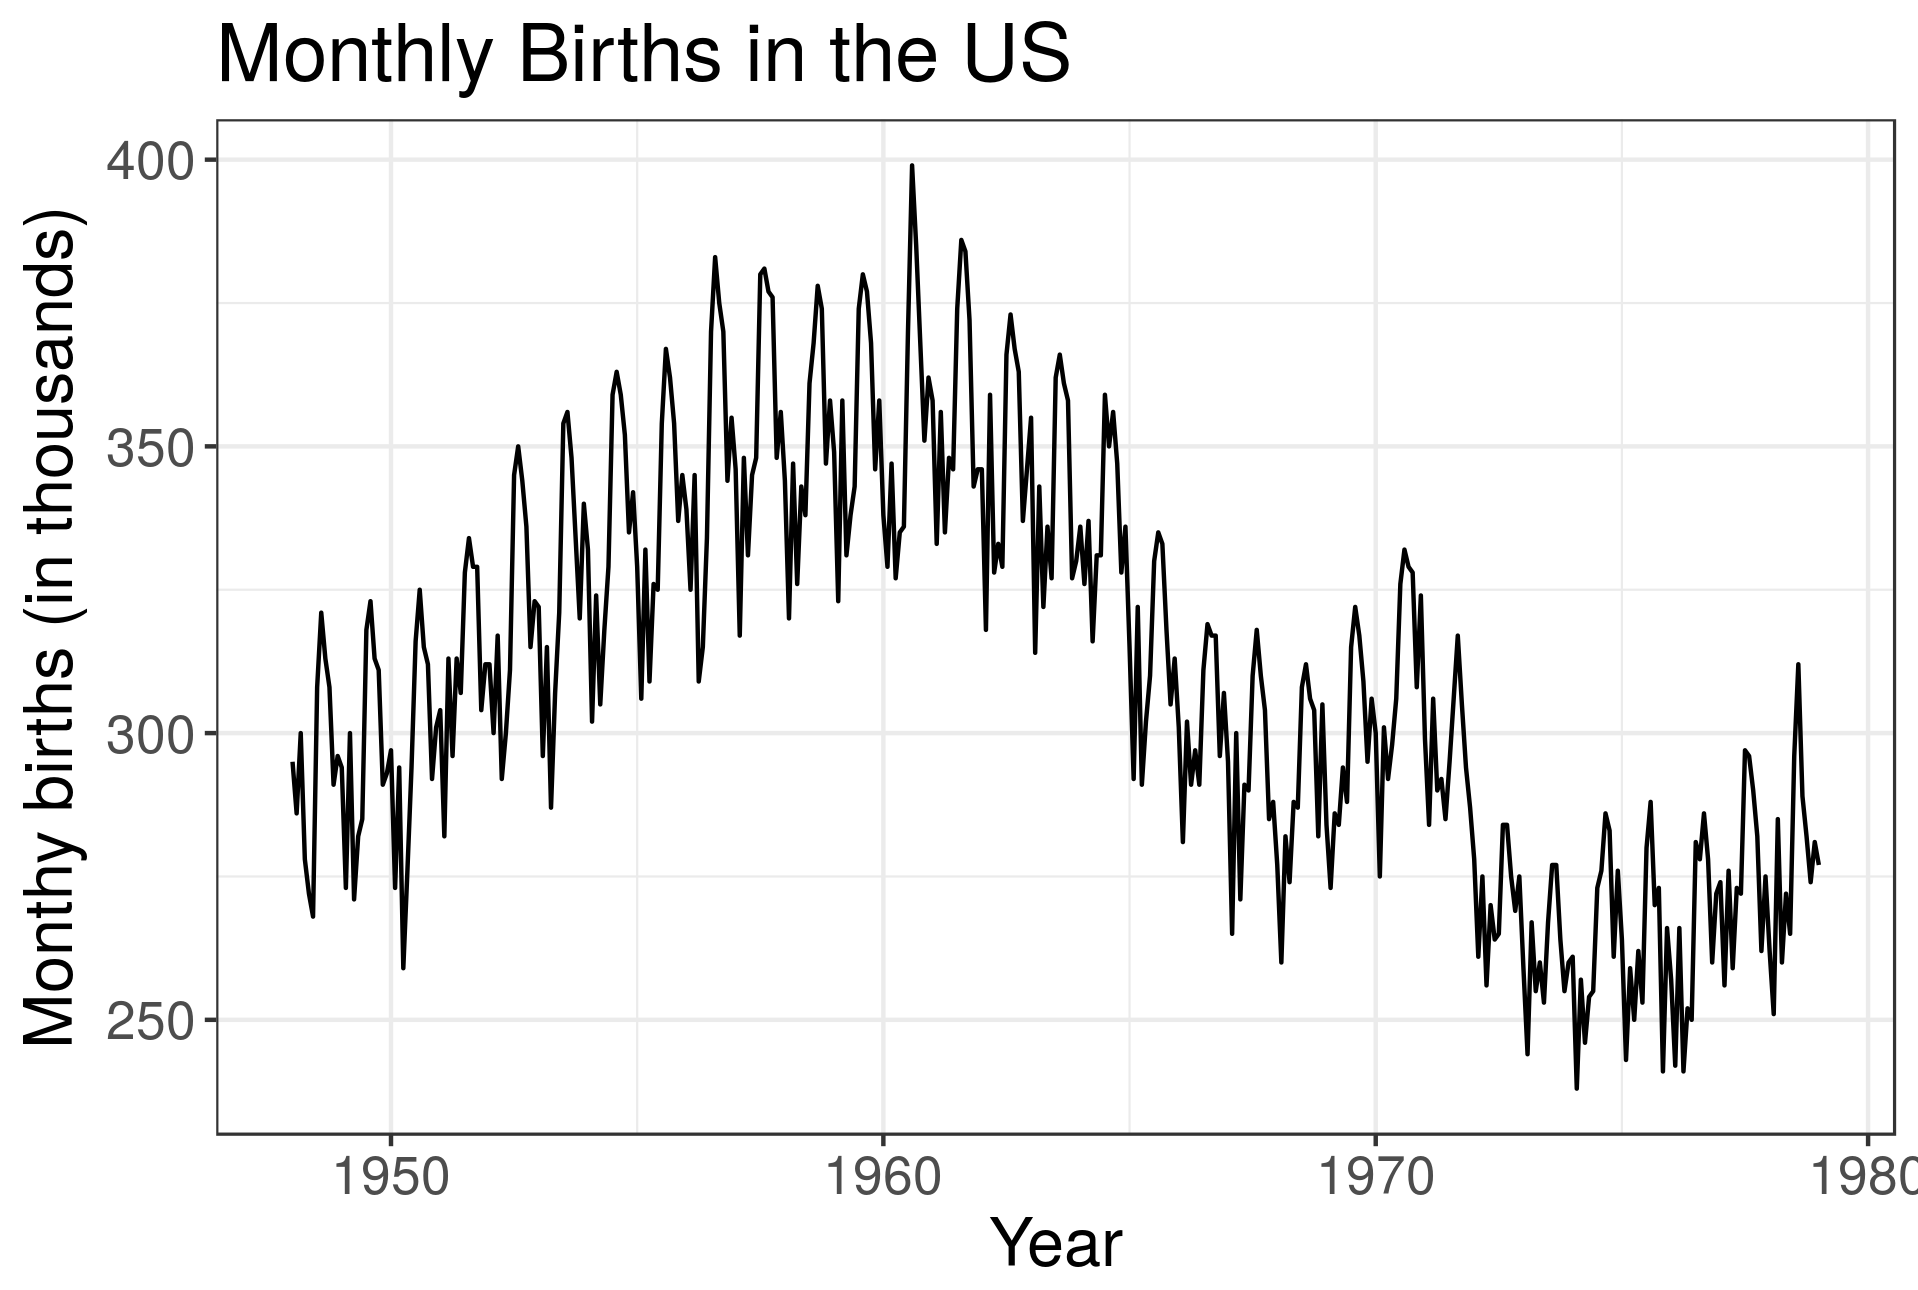
\includegraphics[width = 0.5\textwidth]{./figures/birth_data.png}
	\caption{This is a figure. All figures should be captioned in the document.
	In the figure itself, axes should be properly labeled, and the font legible. }
	\label{fig:birth_data}
\end{figure}

Now to apply the ARIMA models learned in this class, you must make this data
stationary. More plots should follow to justify why your transforms have worked.
By the end of this section, you should have a transformed time series $Y_t$
that is stationary.

\section{Frequency Domain Analysis}\label{sec:FDA}
In this section, you will analyze the data in the Fourier domain to see if you
can detect any seasonalities. Figure~\ref{fig:fd_analysis} is yet another example of
how to insert plots
in LaTex. Here, we demonstrate how to use subplots in LaTex, in
case you may want to put two (or more) plots together.

\begin{figure}[h!]
    \centering
    \begin{subfigure}[b]{0.45\textwidth}
			\centering
        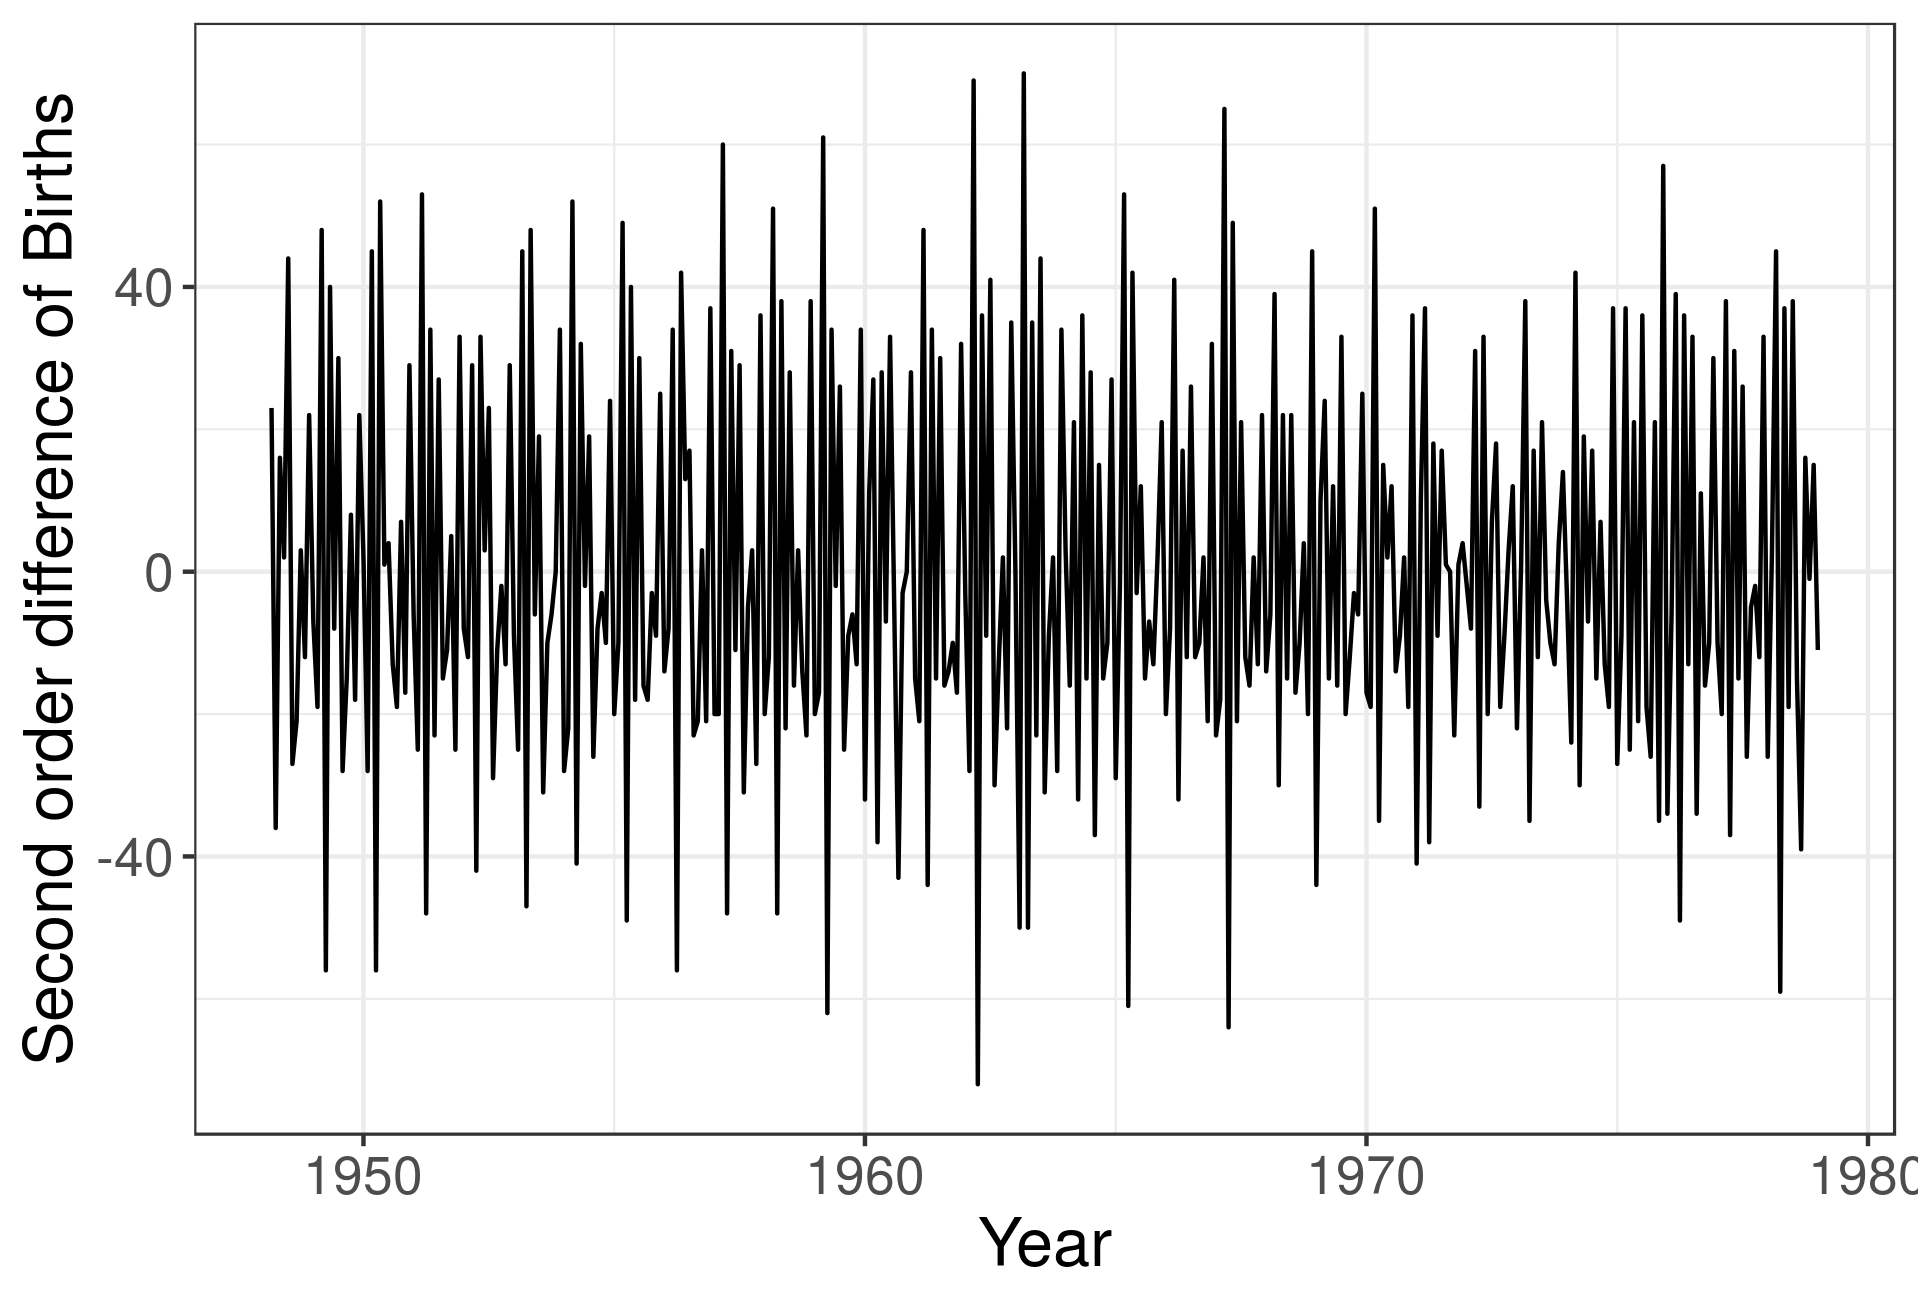
\includegraphics[width=\textwidth]{./figures/diff2_birth_data.png}
        \caption{The second order differences. }
        \label{fig:diff2_birth}
    \end{subfigure}
    ~ %add desired spacing between images, e. g. ~, \quad, \qquad, \hfill etc.
      %(or a blank line to force the subfigure onto a new line)
    \begin{subfigure}[b]{0.45\textwidth}
			\centering
        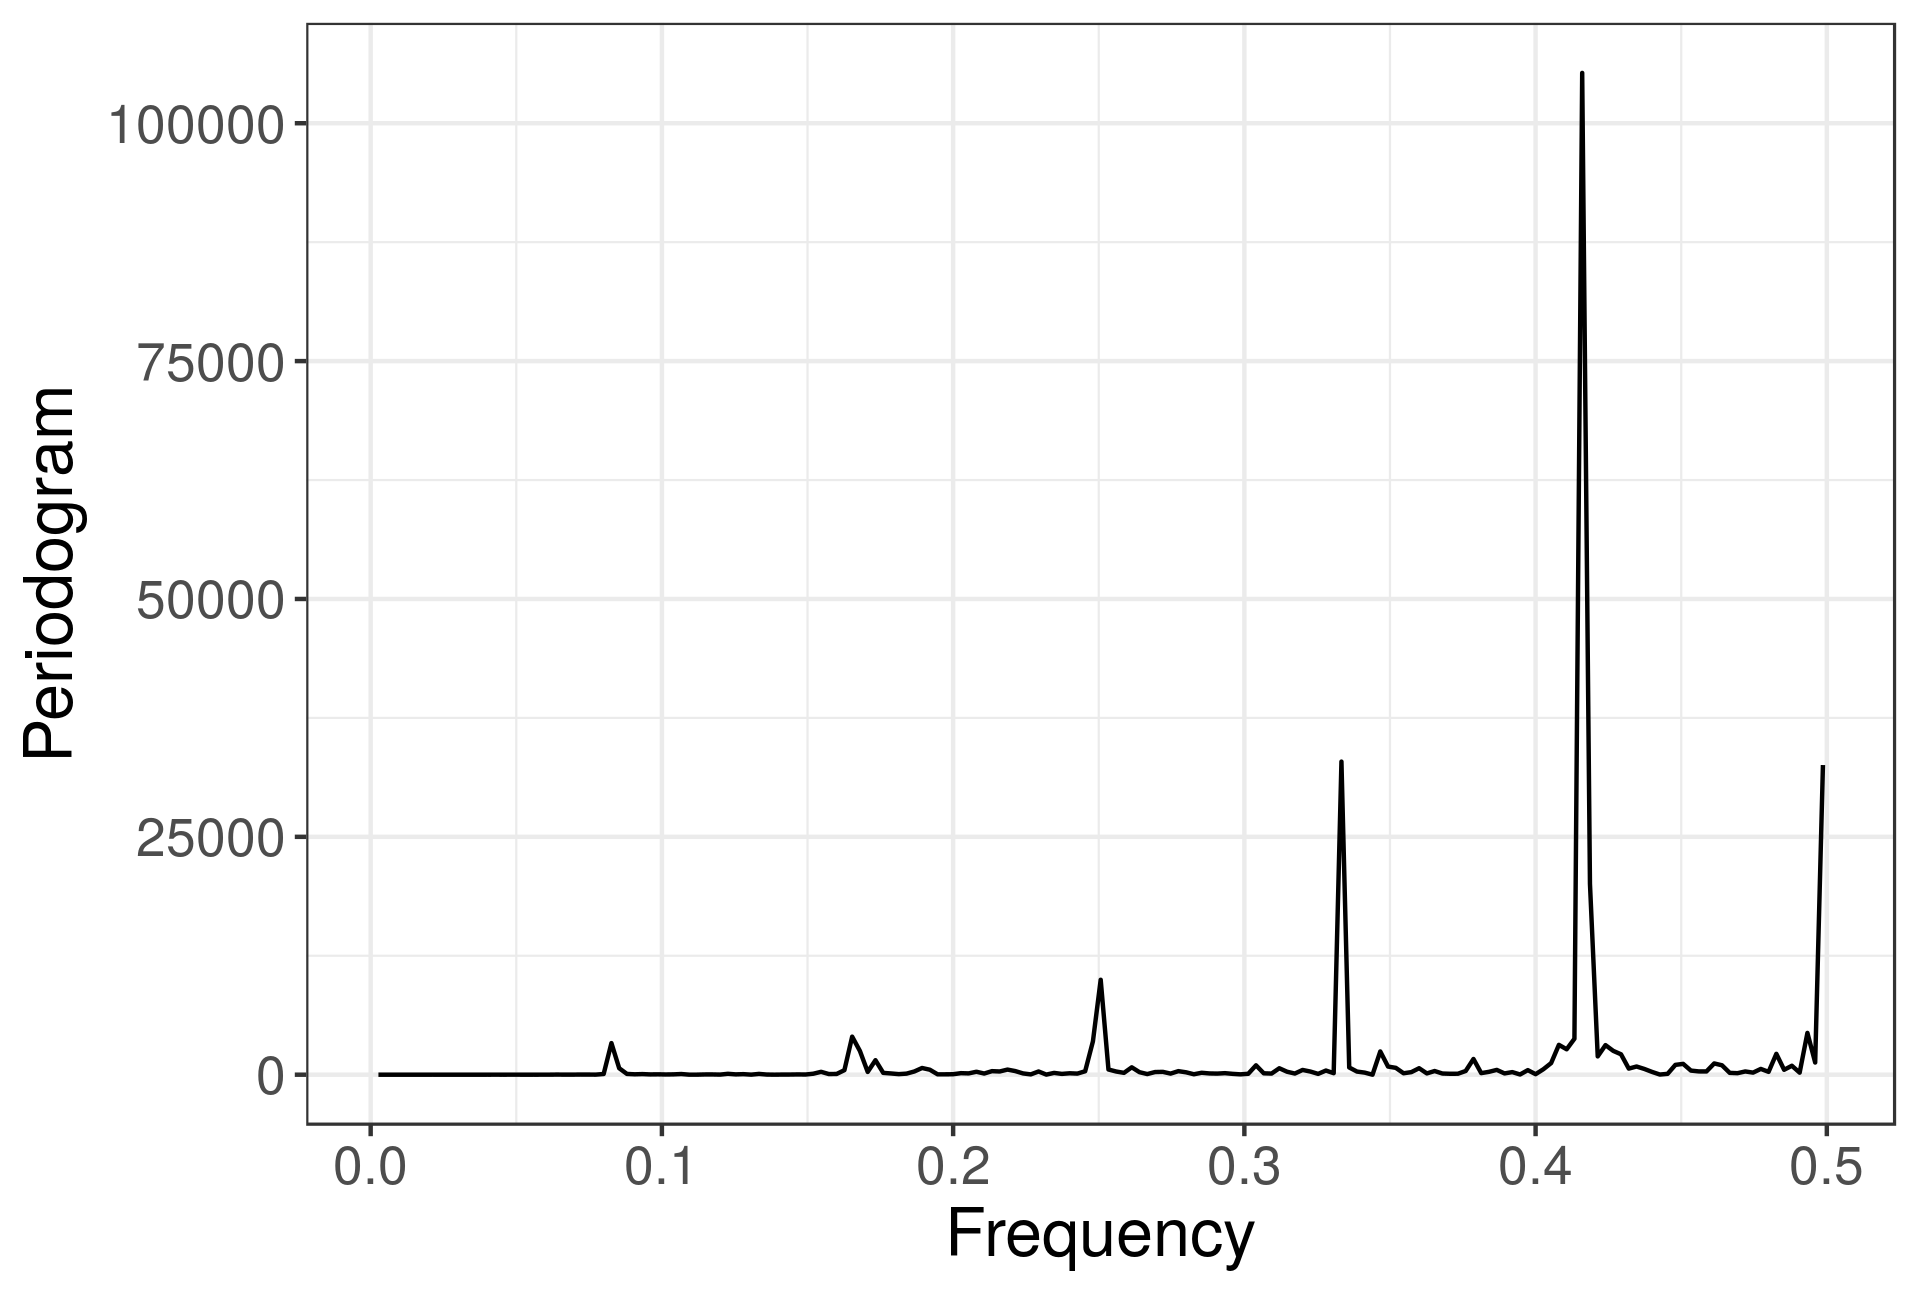
\includegraphics[width=\textwidth]{./figures/diff2_birth_pdg.png}
        \caption{A periodogram of the second order differences. }
        \label{fig:diff2_birth_pdg}
    \end{subfigure}
		\caption{An example of subplots in
		LaTex. Frequency analysis of the second order difference of monthy births. }
		\label{fig:fd_analysis}
\end{figure}

Sometimes it can be a bit tricky to get figures in Latex placed in the position you want them to be. The command \texttt{$\backslash$FloatBarrier} might be useful.

\FloatBarrier

\section{ARIMA Model Selection}
\label{sec:arima_model}
In this section, you derive an ARIMA (or SARIMA, MSARIMA, etc.) model, which you use in Section \ref{sec:results} to make predictions. 
%
On the way, you should compare different candidate models and do diagnostics for them. 
%
Go through the lecture materials and try your best to apply all the different approaches to find models, evaluate their accuracy, and make comparison between different models.
%
At the end of this section you should have decide for \textbf{one single model} you want to work with for your analysis. You may also want to consider other models than ARIMA, e.g., a regression approach based on Section \ref{sec:FDA}. 
%
%
%Sometimes, it may be helpful to introduce subsections.
%\subsection{Cross Validation Model Comparison}
%For example, you may want to compare different models by how well the predict future values (as your predictions will also be evaluated in this final project).

%Lets leave out year 1978 when fitting models, and hold that as a test set. A
%table and some figures might be in order. Table~\ref{tab:mse} shows our
%train and test MSE on the three models
%discussed in section~\ref{sec:arima_model}. Figure~\ref{fig:birth_pred} shows our predictions for year 1975 to 1979 using
%our ARIMA model.

%\begin{table}[h!]
%	\centering
%	\begin{tabular}{l|r|r}
%	  Model & Train MSE & Test MSE \\ \hline
%	  model1 & 0.21 & 0.24\\
%	  model2 & 0.18 & 0.26 \\
%		model3 & 0.34 & 0.4 \\
%	\end{tabular}
%	\caption{MSE on the training set and the test set for the three models
%	discussed in section~\ref{sec:arima_model}. }
%	\label{tab:mse}
%\end{table}


%\begin{figure}[h!]
%	\centering
%	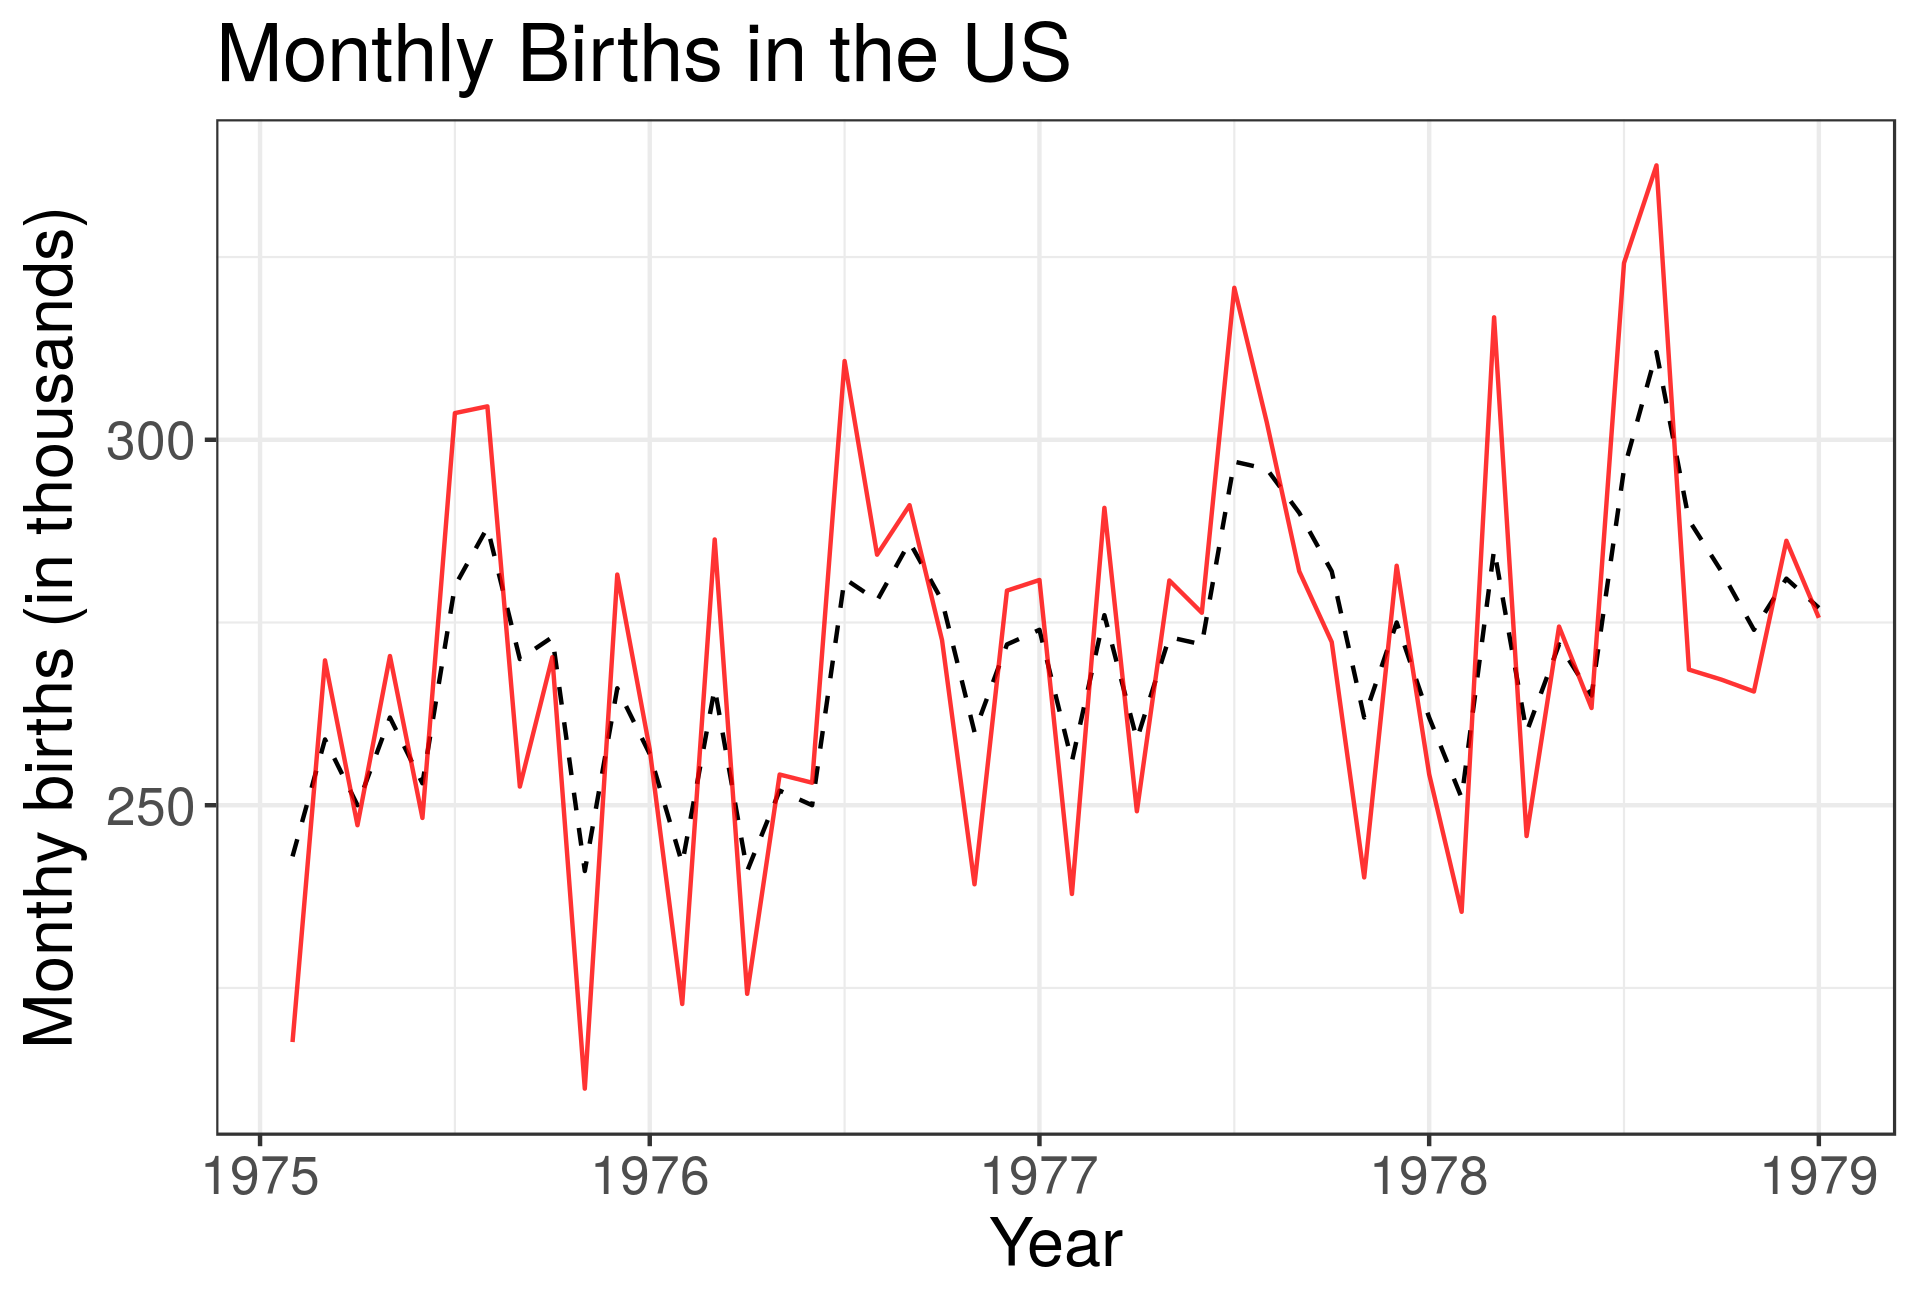
\includegraphics[width = 0.6\textwidth]{./figures/birth_predictions.png}
%	\caption{Predictions of birth data (in red) against the true data (black). }
%	\label{fig:birth_pred}
%\end{figure}



\section{Results}\label{sec:results}
Here, you will discuss the results of your model fit from
Section~\ref{sec:arima_model}. 
%
Math is very easy in Latex. Our ARIMA
model is defined in equation (\ref{eq:first_arma_model}). See how I referenced the
equation in LaTex?
\begin{align}
	(1 - \phi_1 B - \phi_2B^2) \nabla^2 X_t = (1 - \theta_1 B)W_t
	\label{eq:first_arma_model}
\end{align}
Perhaps some subsections will help the organization.
%
\subsection{Estimation of model parameters }
This might be a good time to introduce tables
in LaTex (Table~\ref{tab:param_est}).
All tables should be captioned, accordingly.

\begin{table}[h!]
	\centering
	\begin{tabular}{l|r}
	  Parameter & Estimate (s.e) \\ \hline
	  $\phi_1$& -0.29 (0.06) \\
	  $\phi_2$ & 0.068 (0.05) \\
		$\theta_1$ & -0.99(0.007)
	\end{tabular}
	\caption{These are our parameter estimates and corresponding standard errors
	for the ARIMA model in
	equation~\ref{eq:first_arma_model}. }
	\label{tab:param_est}
\end{table}
\newpage
\subsection{Prediction}
Every group will be providing estimates of future values that are not in the dataset, and there will be one submission PER GROUP.
Only the instructor will have values, and we will be evaluating your models.\\
\\
\textbf{Prediction File Submission:}\\
\\
For each of the three datasets, you'll be submitting a text file of predictions, separated by commas. For a dataset, the prediction file's name should be in the following format:
\begin{center}
    D[\# of dataset]\_[Group \#]\_[SID member 1]\_[SID \#2]\_[SID \#3]\_[SID \#4]\_[SID \#5].csv
\end{center}
You can view your group numbers on the posted Excel spreadsheet in bCourses. If your group doesn't have 5 members, then the remaining SID slots should be "NA". For example, if Merle, Brian, and Frank are in Group 0 submitting predictions for dataset 2, then the file name would be :
\begin{center}
    D2\_0\_1234\_2345\_3456\_NA\_NA.csv
\end{center}
**bCourses will have a sample submission for reference as well as an R script, "file\_reader", for you to check if your file will be read correctly.




\end{document}
\grid
